\chapter{Implementasi dan Pengujian}
\label{chap:implementasiPengujian}

Bab ini terdiri atas dua bagian, yaitu Implementasi Perangkat Lunak dan Pengujian Perangkat Lunak. Bagian implementasi berisi penjelasan lingkungkan pengembangan perangkat lunak dan hasil implementasi. Sedangkan bagian pengujian berisi hasil pengujian fungsional dan eksperimental terhadap perangkat lunak yang telah dibangun.

\section{Implementasi}
\label{sec:implementasi}

\subsection{Lingkungan Implementasi}
		\label{sec:lingkungan_implementasi}
			Implementasi perangkat lunak ini dilakukan di satu buah komputer. Implementasi pertama dilakukan pada komputer peneliti untuk keperluan pengujian fungsional. Komputer tersebut memiliki spesifikasi sebagai berikut:
				\begin{enumerate}
					\item Processor: 2.80Ghz 
					\item RAM: 16.00 GB DDR4	
					\item Sistem Operasi: Windows 10 Pro 64-bit 
					\item Versi Java: 1.8.0\_181
				\end{enumerate}
				
\subsection{Hasil Implementasi}
		Hasil implementasi berupa aplikasi berbasis web yang dikembangkan untuk menyesuaikan dengan StudentPortal Baru dan Kurikulum 2018. Aplikasi dapat diakses dengan URL \url{https://ifstudentportalskripsi.herokuapp.com}. Aplikasi Informatika Student Portal terdiri dari lima halaman antara lain:
		\begin{enumerate}
			\item\textbf{Halaman \textit{Login}}\\
				Halaman \textit{login} digunakan pengguna untuk masuk ke dalam aplikasi. Pada halaman ini, pengguna dapat melakukan \textit{login} dengan mengisi \textit{email} pada kolom \textit{email} dan \textit{password} pada kolom \textit{password} kemudian mengklik tombol login. Tangkapan layar dari halaman \textit{login} dapat dilihat pada Gambar \ref{fig:5_halaman_login}.
					\begin{figure}[H]
						\centering
						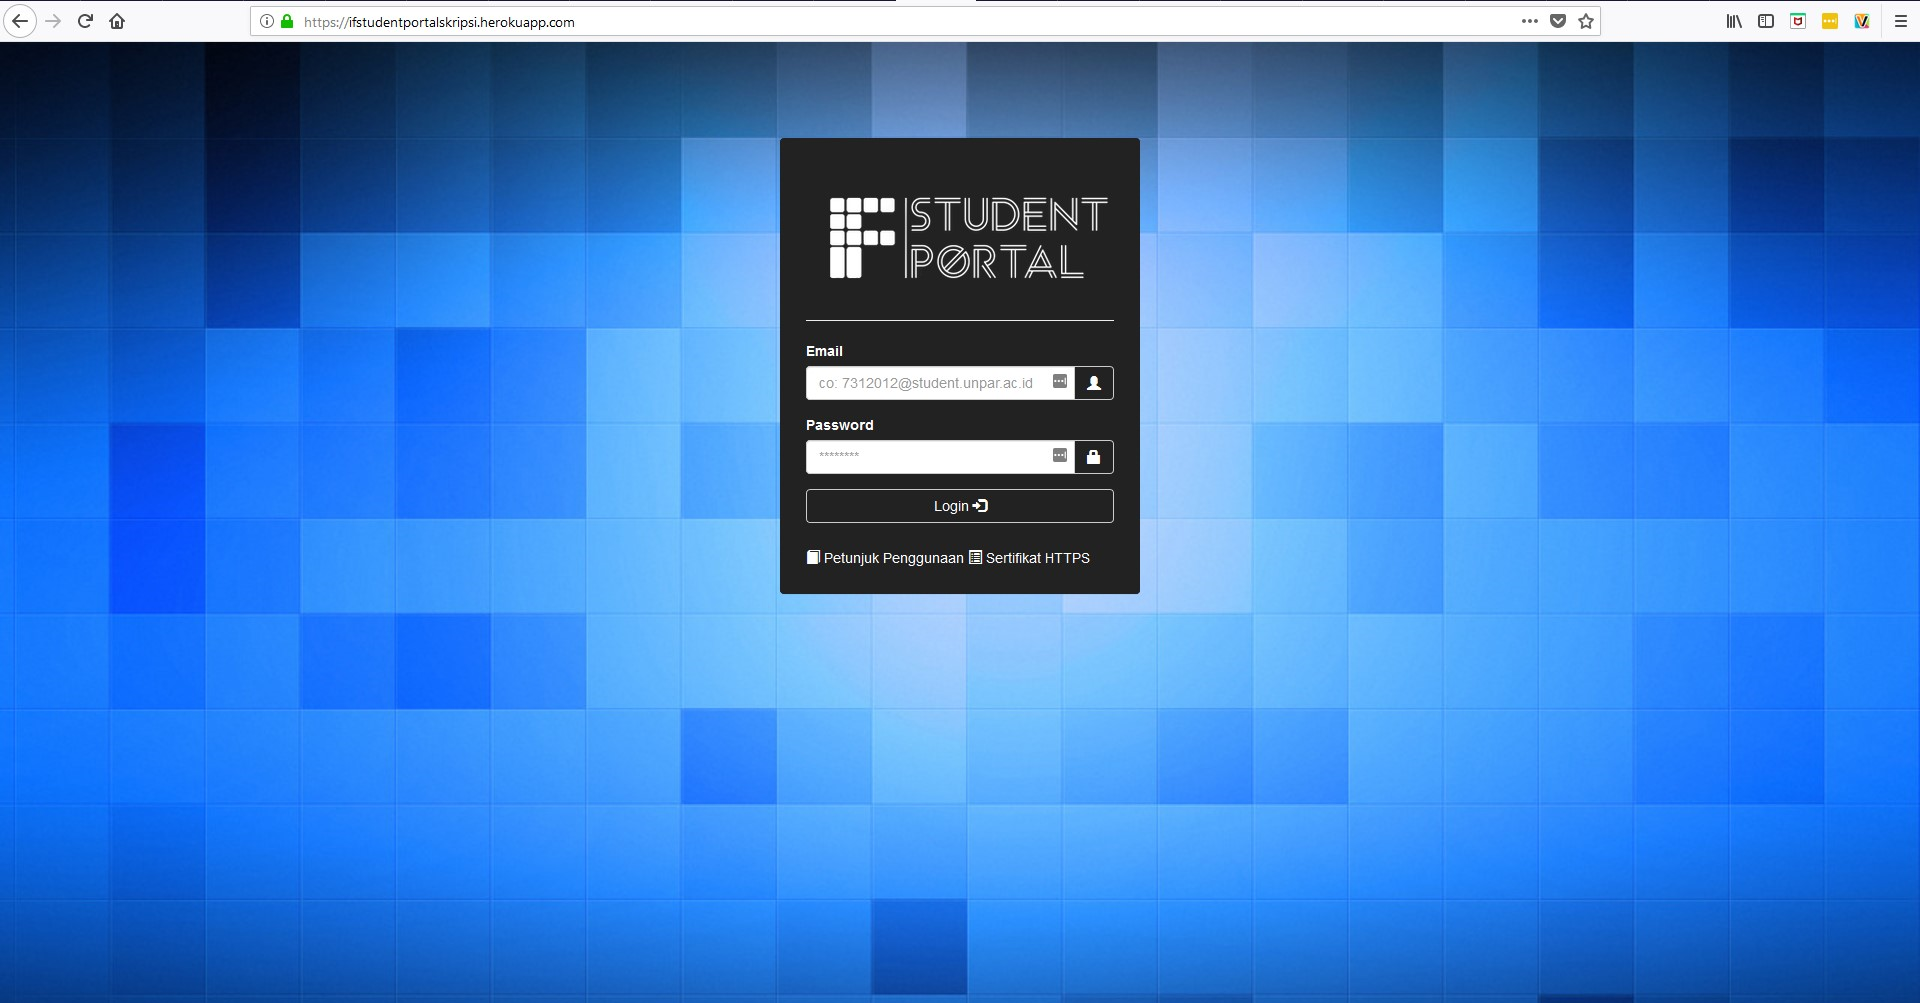
\includegraphics[scale=0.34]{Gambar/halaman_login}
						\caption{Halaman \textit{Login}} 
						\label{fig:5_halaman_login}
					\end{figure}
					
				\item\textbf{Halaman \textit{Home}}\\
				Halaman utama merupakan halaman yang pertama kali dituju setelah melakukan \textit{login}. Halaman utama menampilkan identitas pengguna dan \textit{link} menuju kode sumber aplikasi Informatika Student Portal. Tangkapan layar dari halaman utama dapat dilihat pada Gambar \ref{fig:5_halaman_utama}.
					\begin{figure}[H]
						\centering
						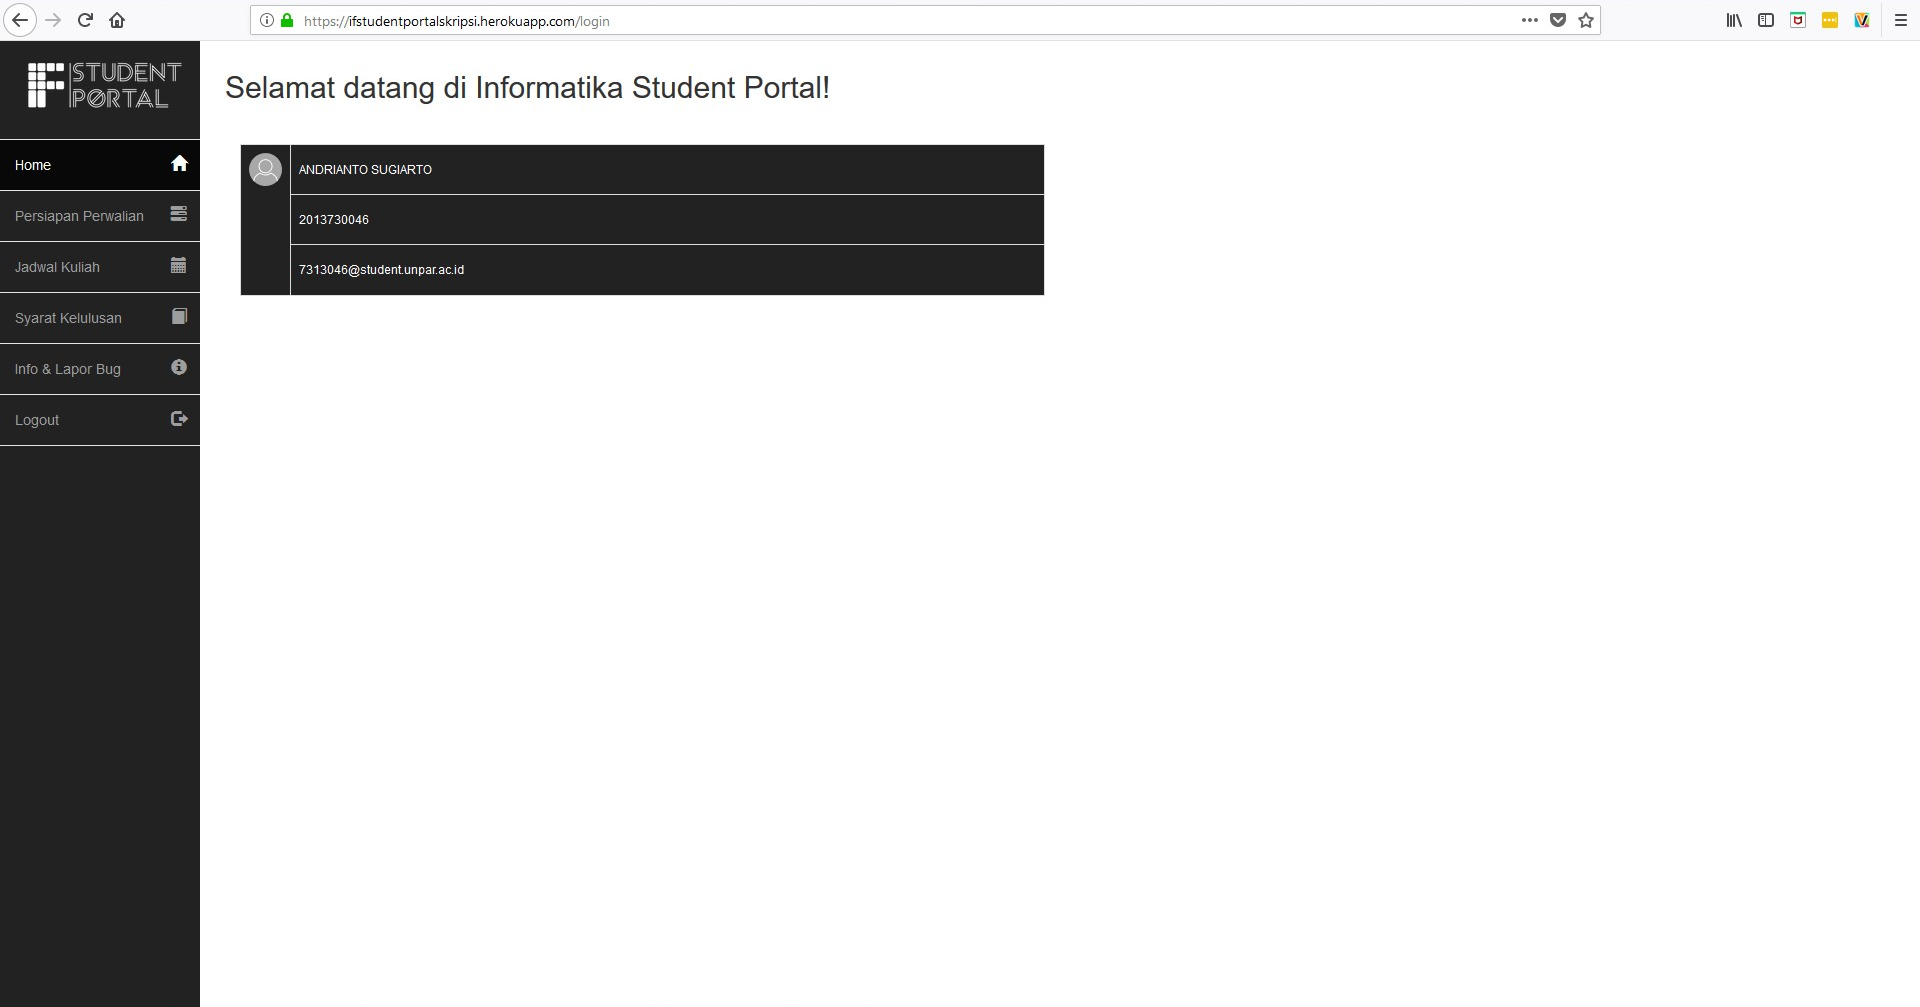
\includegraphics[scale=0.34]{Gambar/halaman_home}
						\caption{Halaman \textit{Home}} 
						\label{fig:5_halaman_utama}
					\end{figure}
						
				\item\textbf{Halaman Persiapan Perwalian}\\
				Halaman ini menampilkan data akademik dan tabel prasyarat mata kuliah. Pengguna dapat mengklik kode mata kuliah, kemudian akan diarahkan ke kode sumber aturan prasyarat mata kuliah tersebut. Tangkapan layar dari halaman prasyarat mata kuliah dapat dilihat pada Gambar \ref{fig:5_halaman_persiapan_perwalian}.
					\begin{figure}[H]
						\centering
						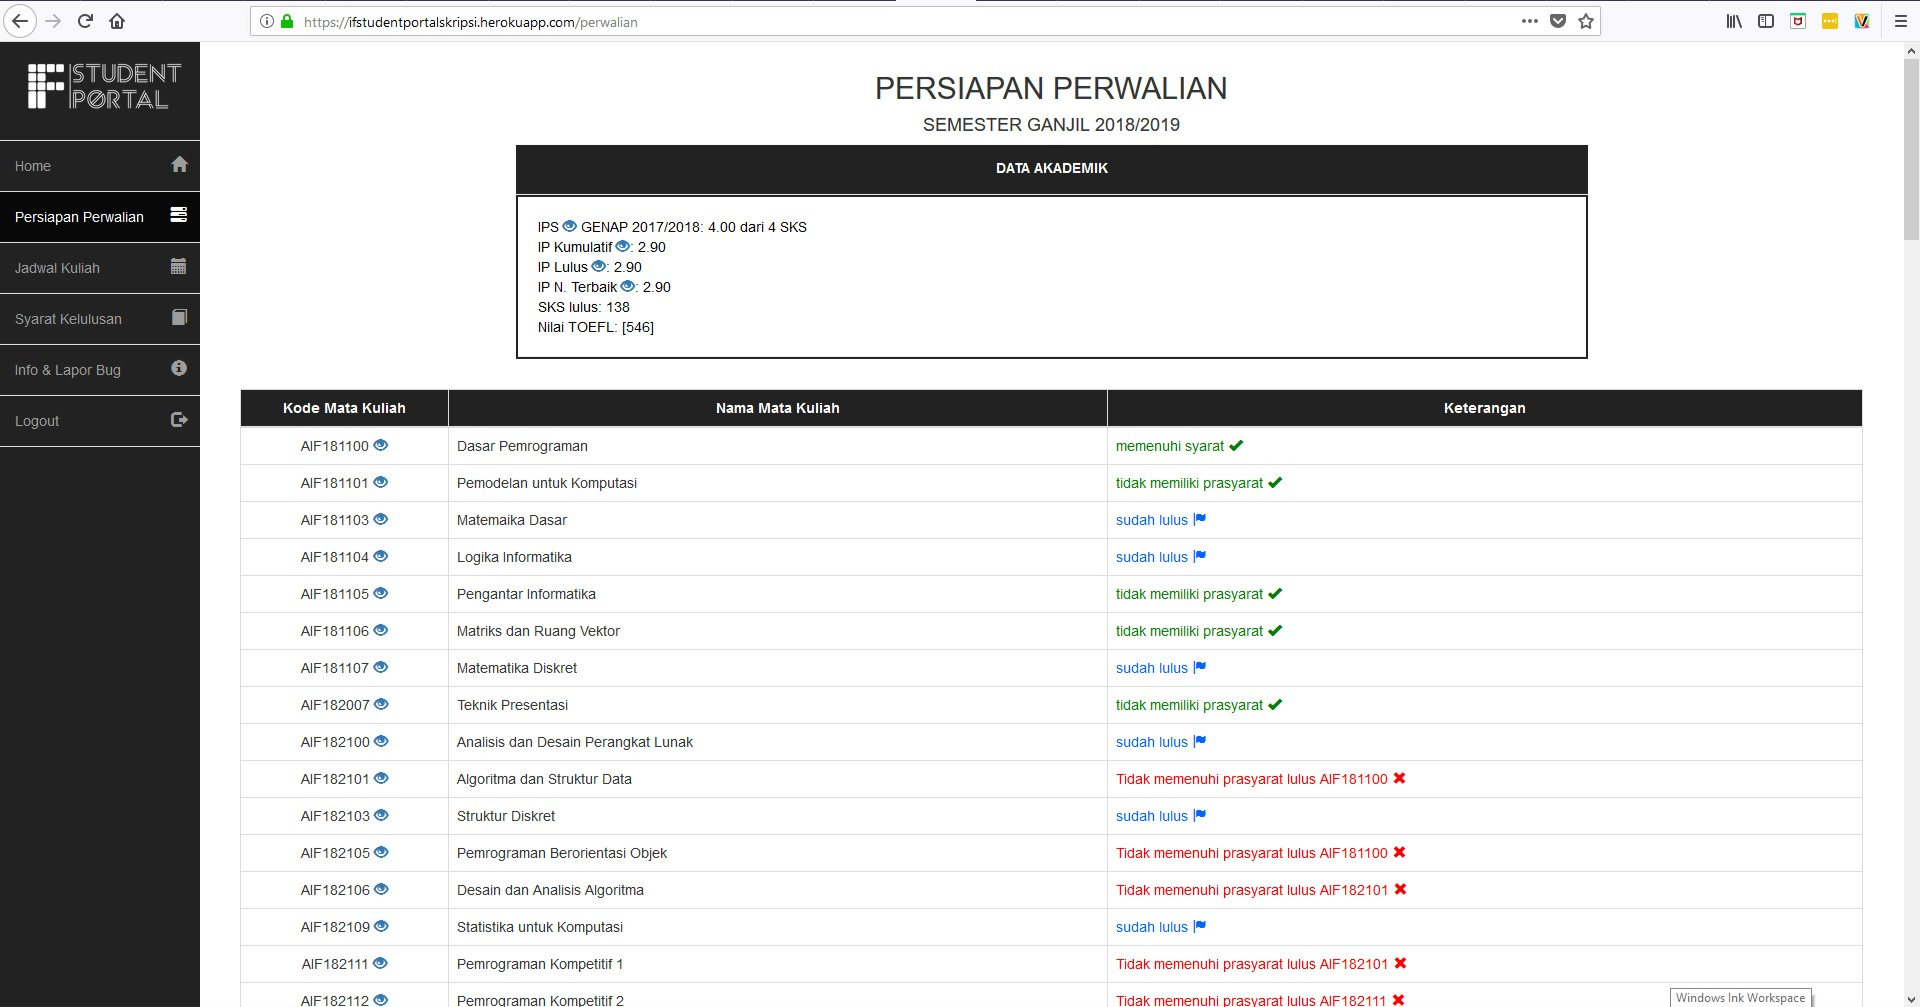
\includegraphics[scale=0.34]{Gambar/halaman_persiapan_perwalian}
						\caption{Halaman Persiapan Perwalian} 
						\label{fig:5_halaman_persiapan_perwalian}
					\end{figure}

				\item\textbf{Halaman Jadwal Kuliah}\\
				Halaman ini menampilkan jadwal kuliah yang tersusun dan terurut berdasarkan hari. Tangkapan layar dari halaman jadwal kuliah dapat dilihat pada Gambar \ref{fig:5_halaman_jadwal}. Jika kode mata kuliah diklik, akan muncul \textit{popup} seperti pada Gambar \ref{fig:5_halaman_jadwal_rinci} yang berisi rincian dari jadwal kuliah tersebut.
				\begin{figure}[H]
						\centering
						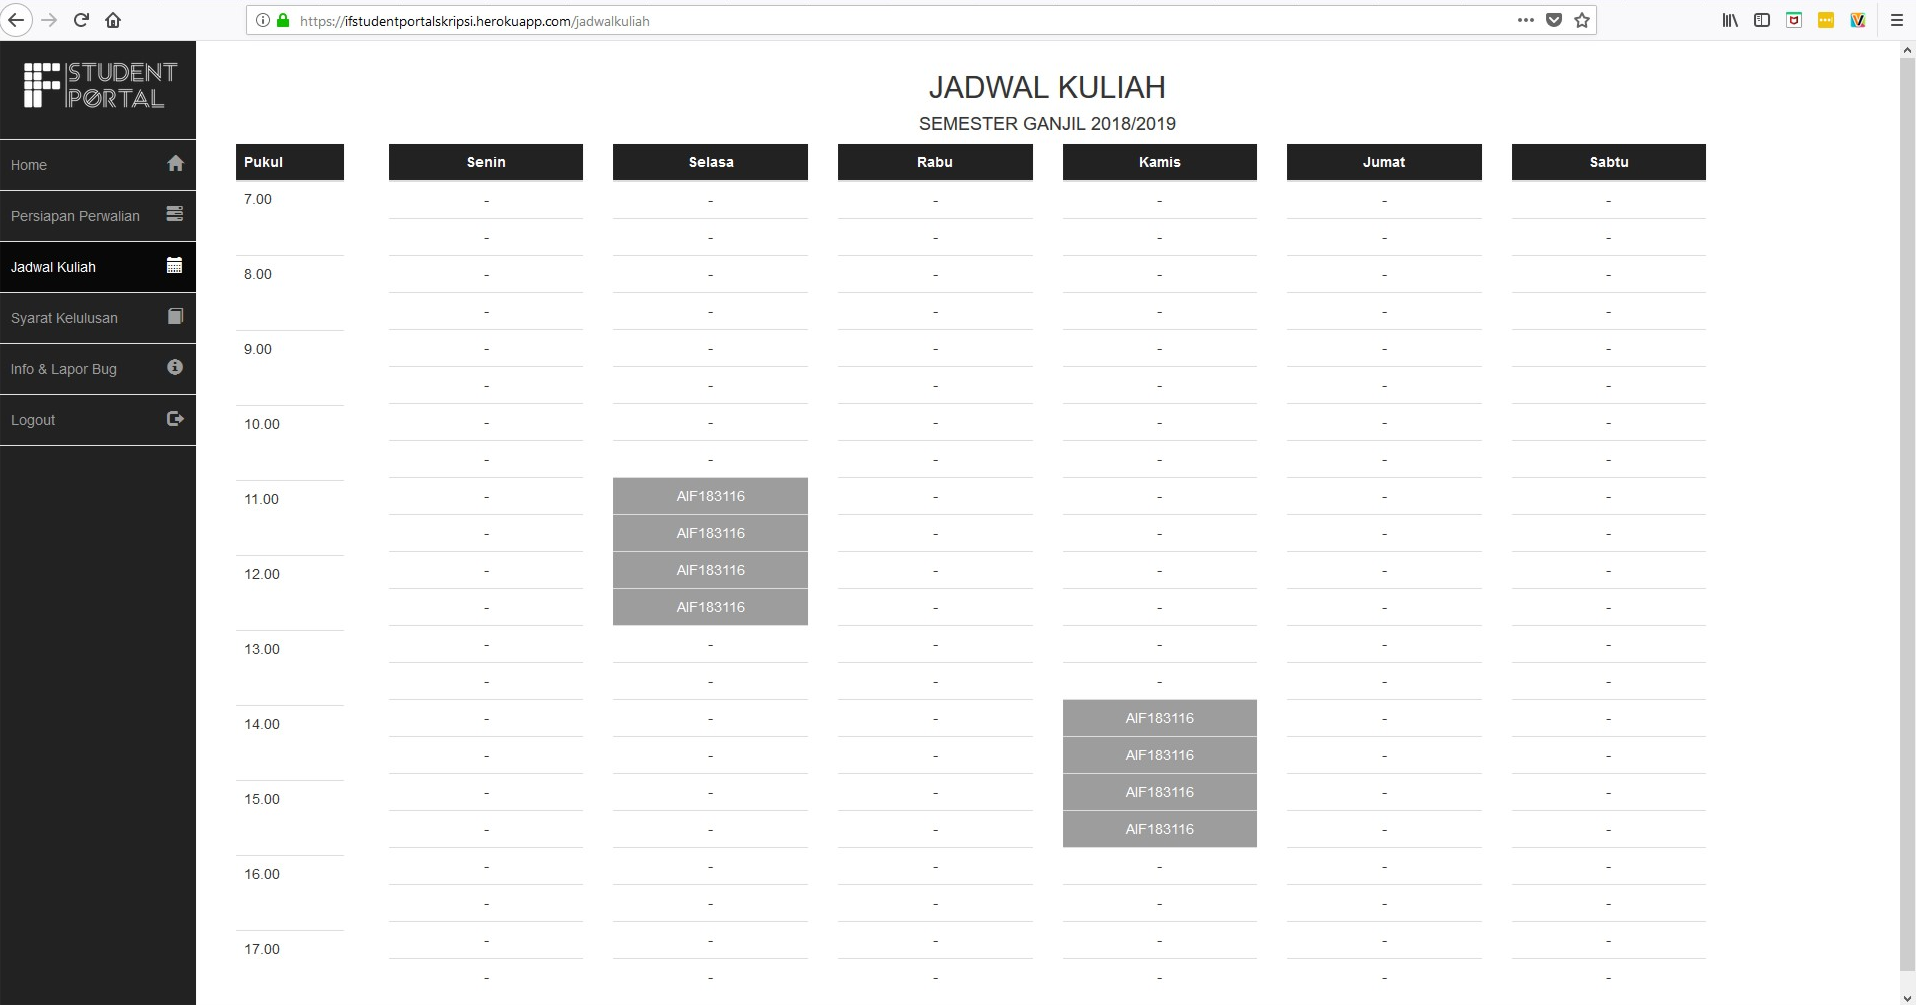
\includegraphics[scale=0.34]{Gambar/halaman_jadwal}
						\caption{Halaman Jadwal Kuliah} 
						\label{fig:5_halaman_jadwal}
					\end{figure}
					
					\begin{figure}[H]
						\centering
						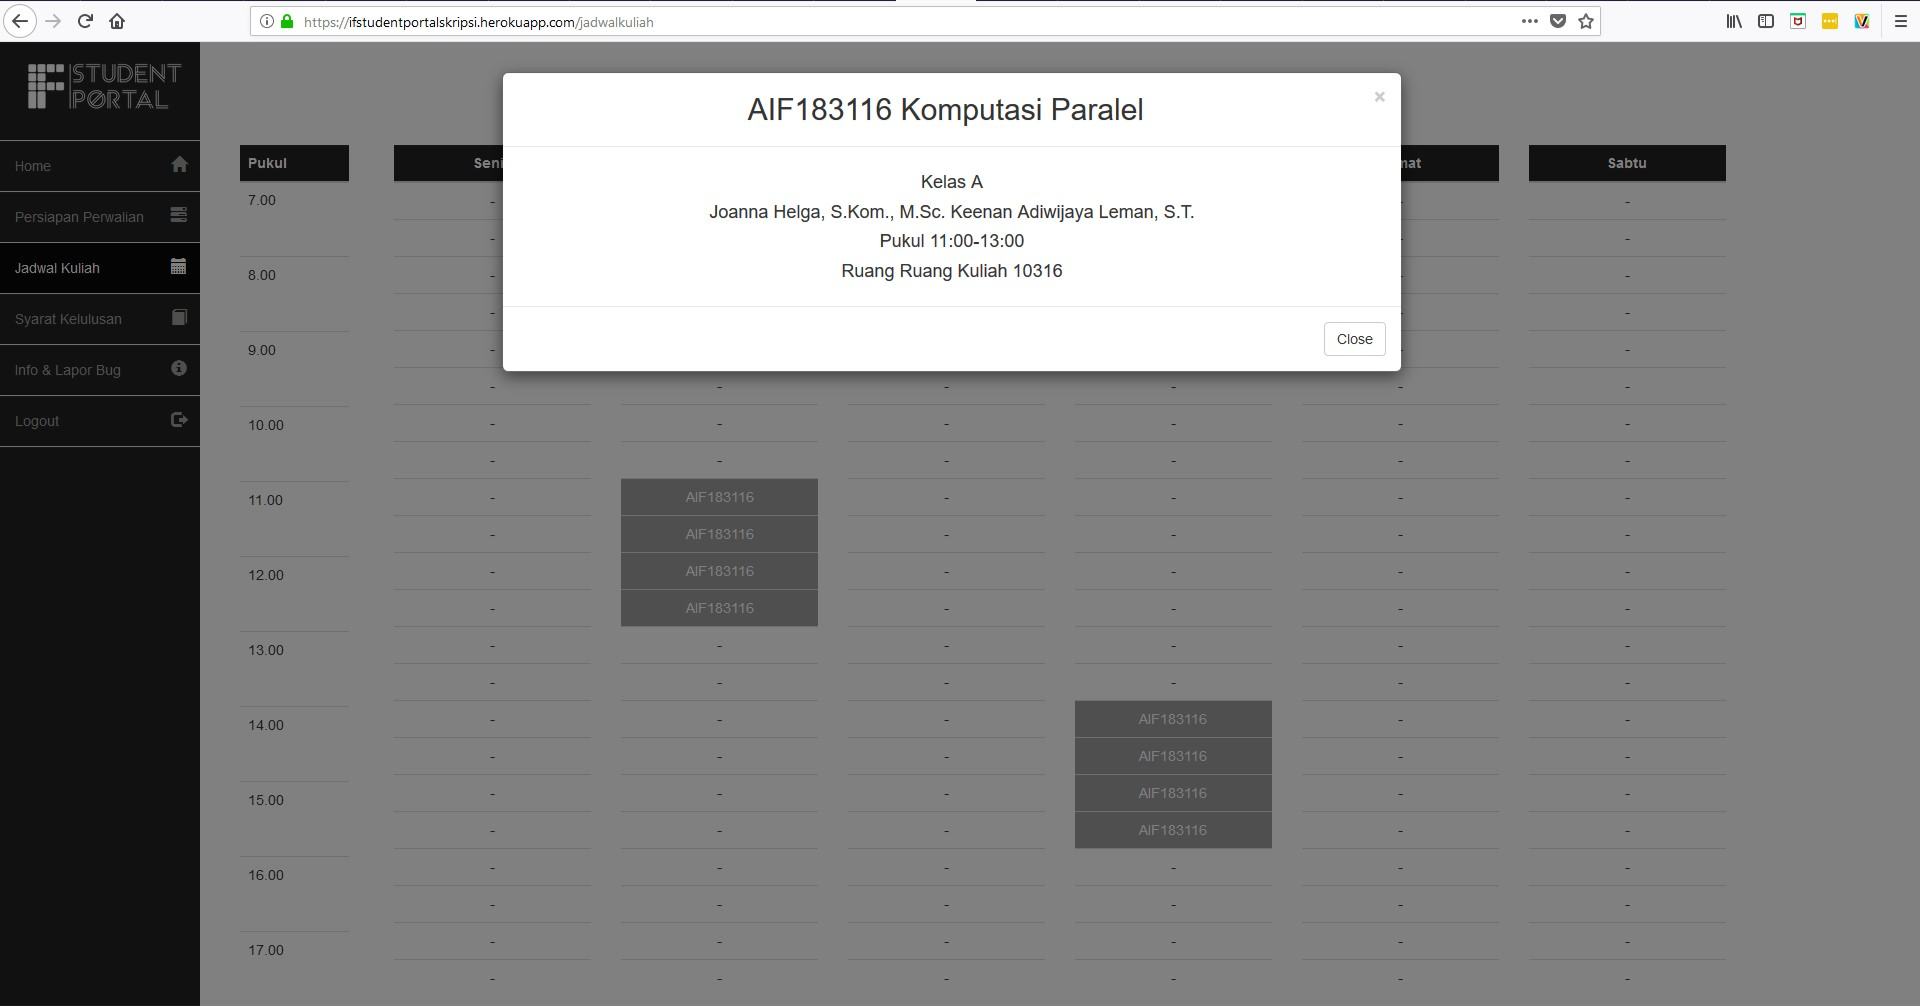
\includegraphics[scale=0.34]{Gambar/halaman_jadwal_rinci}
						\caption{Rincian Jadwal Kuliah} 
						\label{fig:5_halaman_jadwal_rinci}
					\end{figure}
					
				\item\textbf{Halaman Syarat Kelulusan}\\
				Halaman ini menampilkan syarat kelulusan dari Program Studi Teknik Informatika yang belum dipenuhi oleh mahasiswa. Tangkapan layar dari halaman data akademik dapat dilihat pada Gambar \ref{fig:5_halaman_syarat_kelulusan}.
				\begin{figure}[H]
						\centering
						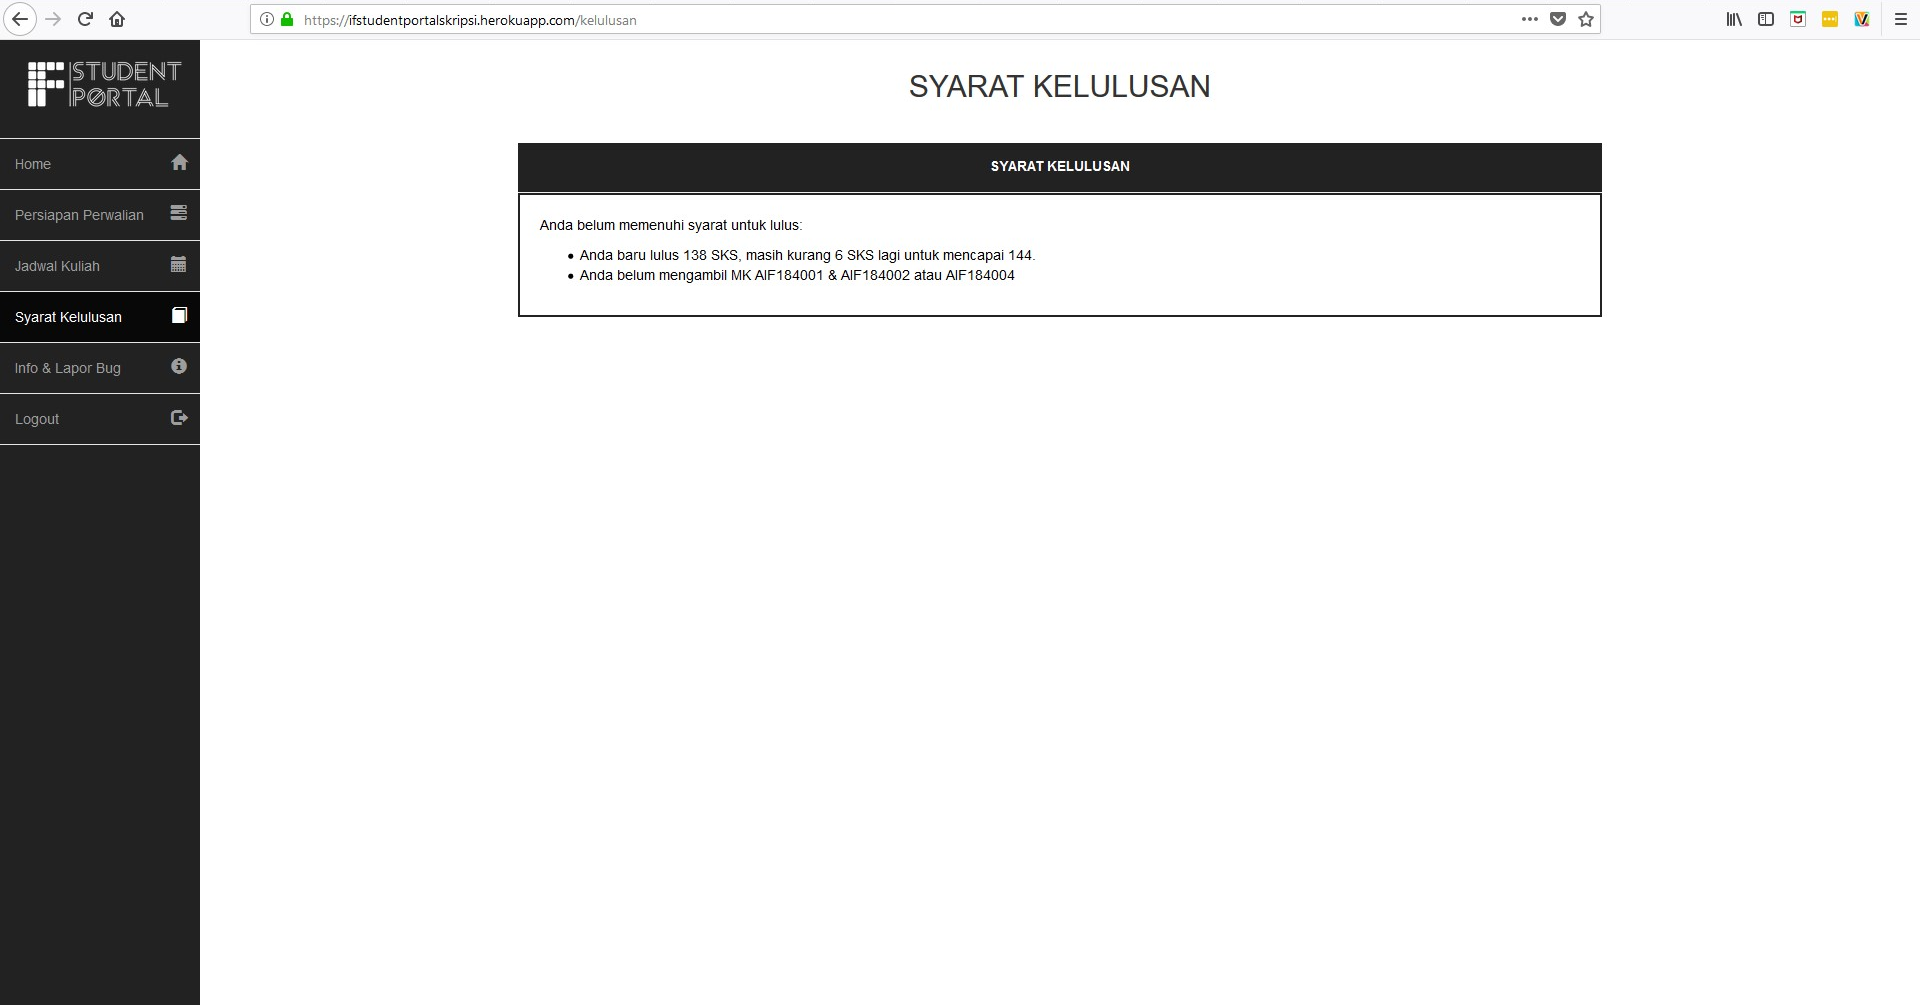
\includegraphics[scale=0.34]{Gambar/halaman_syarat_kelulusan}
						\caption{Halaman Syarat Kelulusan} 
						\label{fig:5_halaman_syarat_kelulusan}
					\end{figure}
		\end{enumerate}
		
\section{Pengujian}